\documentclass[12pt, oneside]{report}

\usepackage[left=3.5cm, top=2.5cm, bottom=2.5cm, right=2.5cm]{geometry}

\usepackage[utf8]{inputenc}
\usepackage[T1]{polski}
\usepackage[polish]{babel}
\usepackage{indentfirst}
\usepackage{graphicx}

\usepackage{natbib}


\begin{document}  
\thispagestyle{empty}
\begin{titlepage}
    \begin{center}

           \Large
	\textbf{Uniwersytet Jagielloński w Krakowie}\vspace{0.2cm}\\ Wydział Fizyki, Astronomii i Informatyki Stosowanej
               \vspace*{1cm}
               
         \vspace{3cm}
         \Large
          \textbf{Paweł Sławomir Mstowski}\\\vspace{0.5cm}
         \normalsize Nr albumu: 1148921\\
             \vspace{2cm}
        \Huge
        \textbf{Nauczanie sieci neuronowych za pomocą algorytmu genetycznego na przykładzie samouczącego się bota do gry zręcznościowej.}
      
        \vspace{1.5cm}
        \normalsize
        Praca magisterska\\
        na kierunku Informatyka Stosowana\\ \vspace{0.15cm}
        
        \vfill
        \vspace{2cm}
       \begin{minipage}{1\textwidth}
\begin{flushright}
Praca wykonana pod kierunkiem\\
prof. dr hab. Piotra Białasa\\
Zakład Technologii Gier
\end{flushright}
\end{minipage}
        
        \vspace{2cm}
        \begin{center}
      Kraków 2019
        \end{center}
    \end{center}
\end{titlepage}

\newpage 
 \thispagestyle{empty}
\vspace{2.5cm}
\begin{flushleft}
\large \textbf{Oświadczenie autora pracy}\vspace{0.6cm}\\
\end{flushleft}

\noindent Świadom odpowiedzialności prawnej oświadczam, że niniejsza praca dyplomowa została napisana przeze mnie samodzielnie i nie zawiera treści uzyskanych w sposób niezgodny z obowiązującymi przepisami.\\

\noindent Oświadczam również, że przedstawiona praca nie była wcześniej przedmiotem procedur związanych z uzyskaniem tytułu zawodowego w wyższej uczelni.
\vspace{2cm}
\begin{center}
\begin{tabular}{lr}
................................~~~~~~~~~~~~~~~~~~~~~~~~~~~~~~~~~~~~~~&
.......................................... \\
{~~~~Kraków, dnia} & {Podpis autora pracy~~~~}
\end{tabular}
\end{center}
\vspace{5cm}
\begin{flushleft}
\large \textbf{Oświadczenie kierującego pracą}
\end{flushleft}

\noindent Potwierdzam, że niniejsza praca została przygotowana pod moim kierunkiem i~kwalifikuje się do przedstawienia jej w postępowaniu o nadanie tytułu zawodowego.
\vspace{2cm}
\begin{center}
\begin{tabular}{lr}
................................~~~~~~~~~~~~~~~~~~~~~~~~~~~~~~~~~~~~~~&
............................................ \\
{~~~~Kraków, dnia} & {Podpis kierującego pracą~~}
\end{tabular}
\end{center}
\vfill
\tableofcontents

%%%%%%%%%%%%%%%%%%%%%%%%%%%%%%%%%%%%%%%%%%%%%%%%%%%%%%%%%%%%%%%%%%%%%%%%%%%%%%%%%%%%%


\chapter{Wprowadzenie}

%%%%%%%%%%%%%%%%%%%%%%%%%%%%%%%%%%%%%%%%%%%%%%%%%%%%%%%%%%%%%%%%%%%%%%%%%%%%%%%%%%%%%

\chapter{Sieci neuronowe}
\section{Czym są sieci neuronowe?}

Sieci neuronowe są to systemy przetwarzania informacji wzorowane na procesach i strukturach obserwowanych w ludzkim mózgu. Pierwszą sztuczną siecią neuronową był perceprton progowy, który został wymyślony w roku 1943 przez Warrena Sturgisa McCullocha i Waltera Pittsa. Wymyślona wtedy koncepcja jest nadal bardzo aktualna i wykorzystywana do dziś. Teraźniejszy poziom zaawansowania komputerów i ich moc obliczeniowa wywołały swego rodzaju renesans badań nad sieciami neuronowymi.

Tak samo jak nasz mózg składa się z setek miliardów komórek neuronowych tak sztuczne sieci neuronowe są tworzone przez setki lub tysiące sztucznych neuronów, które są najmniejszymi elementami przetwarzającymi informację. Są one prymitywną interpretacją sposobu działania prawdziwych, biologicznych neuronów i składają się z wielu wejść oraz jednego wyjścia. Budowa takiego pojedynczego elementu sieci przedstawiona jest poniżej (Rysunek \ref{fig: 2.1}).

\begin{figure}[h]
	\centering
	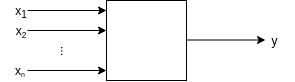
\includegraphics[width=5cm]{fig211.png}
	\caption{Schemat budowy sztucznego neuronu}
	\label{fig: 2.1}
\end{figure}

Każde wejście sztucznego neuronu posiada też swoją wagę, która jest potem używana do obliczenia jego wyjścia. W takim wypadku funkcję każdego pojedynczego elementu sieci możemy zapisać jako

\begin{equation}\label{eq: 2.1}
y = \sum^{n}_{i=1} x_{i}w_{i}
\end{equation}


Topologia połączeń oraz ich parametry stanowią program działania sieci \cite{tadeusiewicz1993sieci}. Sygnały wejściowe są przepuszczane przez chmurę połączonych ze sobą neuronów, które następnie przeliczają te sygnały i przekazują swoje rozwiązania dalej w głąb sieci. Tak przetworzone dane dają w wyniku pewną ilość sygnałów wyjściowych z sieci które razem są rozwiązaniem problemu, do którego została wyuczona.

\section{Zastosowania sieci neuronowych}

Bazując na wcześniej podanych informacjach można powiedzieć, że sztuczne sieci neuronowe pomimo swojej genezy nie są idealnym odzwierciedleniem sposobu działania swojego pierwowzoru, czyli ludzkiego mózgu. Przez swoje ograniczenia ich zdolności do rozwiązywania problemów są ograniczane. Każda sieć neuronowa jest projektowana i uczona do rozwiązywania konkretnego problemu i nie radzi sobie z danymi związanymi z innymi zagadnieniami niż jej specjalizacja.

Z podstaw działania sztucznego neuronu można wywnioskować, że ma on zdolność do rozpoznawania wzorców na podstawie porównania otrzymanych sygnałów do swojego wektora wag. Z tego wynika, że takie neurony połączone w skomplikowaną sieć są idealne do takich zadań na dużo większą skalę. Taki sposób działania pozwala na wykorzystanie tych mechanizmów w wielu branżach.

Aktualnie sieci neuronowe są używane do przetwarzania danych w bardzo dużym spektrum dziedzin. Ich zastosowania można znaleźć przedmiotach codziennego użytku takich jak smartfony, na przykład do rozpoznawania mowy i implementacji interfejsów głosowych, jak też w bardzo profesjonalnych sprzętach i systemach.

Na podstawie wcześniej dostarczonych danych jesteśmy w stanie nauczyć sieci neuronowe przewidywać pewne zdarzenia na podstawie aktualnych danych. Wiele firm w dzisiejszych czasach tworzy systemy, które na podstawie parametrów technicznych urządzeń w zakładach są wstanie podać bardzo dokładne prawdopodobieństwo awarii danego sprzętu.

\section{Metody nauczania}

%%%%%%%%%%%%%%%%%%%%%%%%%%%%%%%%%%%%%%%%%%%%%%%%%%%%%%%%%%%%%%%%%%%%%%%%%%%%%%%%%%%%%

\chapter{Algorytm genetyczny}
\section{Powstanie algorytmu genetycznego}
\section{Problem kodowania rozwiązania}
\section{Zastosowania}

%%%%%%%%%%%%%%%%%%%%%%%%%%%%%%%%%%%%%%%%%%%%%%%%%%%%%%%%%%%%%%%%%%%%%%%%%%%%%%%%%%%%%

\chapter{Wykorzystanie algorytmu genetycznego w nauczaniu sieci neuronowych}

%%%%%%%%%%%%%%%%%%%%%%%%%%%%%%%%%%%%%%%%%%%%%%%%%%%%%%%%%%%%%%%%%%%%%%%%%%%%%%%%%%%%%

\chapter{Samouczący się bot do gry zręcznościowej}
\section{Stos technologiczny}
\section{Struktura projektu}
\section{Zastosowane techniki sztucznej inteligencji}\textsl{}
\section{Opis działania}

\chapter{Wnioski}

\pagebreak
%%%%%%%%%%%%%%%%%%%%%%%%%%%%%%%%%%%%%%%%%%%%%%%%%%%%%%%%%%%%%%%%%%%%%%%%%%%%%%%%%%%%%
\bibliographystyle{plain}
\bibliography{bibliography}
\end{document}